\documentclass[10pt]{article}
\usepackage[margin=0.55in]{geometry}
\usepackage{booktabs,longtable,graphicx,hyperref,xcolor}
\usepackage{array}
\hypersetup{colorlinks=true,linkcolor=blue,urlcolor=blue}
\setlength{\parindent}{0pt}
\setlength{\parskip}{0.45em}

\title{Dynamic Maze Solver Comparison}
\author{HTW EB-JEPA}
\date{20 June 2026}

\begin{document}
\maketitle

\section*{Scope}
This document summarizes the dynamic-maze experiments: symbolic A* baselines,
A*-distilled JEPA subgoal controllers, and A*-free world-model controllers.
Animated GIFs are saved next to this report; the PDF contains static start/end
previews and clickable links to the GIF files.

The table covers 768 closed-loop evaluation episodes across
12 methods. Most rows use 64 episodes. The symbolic/A*-distilled and
bootstrap runs come from different launchers, so oracle-normalized ratios should
be read as operational comparisons rather than as one perfectly matched
benchmark.

\section*{Metric Definitions}
\begin{itemize}
  \item Success is the empirical probability of reaching the goal over 64 episodes.
  \item Runs is the number of closed-loop evaluation episodes available for that method.
  \item Steps is the mean number of executed moves.
  \item Blocked moves counts attempted moves into walls/closed doors.
  \item A* efficiency is the evaluator's per-episode \(A_0/\max(\mathrm{steps}, A_0)\), when available.
  \item Step/oracle is \(\mathrm{mean\ oracle\ steps}/\mathrm{mean\ solver\ steps}\).
  \item Combined is success times Step/oracle; it rewards both reaching the goal and doing so efficiently.
\end{itemize}

\section*{Results}
\small
\begin{longtable}{p{0.24\linewidth}rrrrrrr}
\toprule
Method & Runs & Success & Steps & Blocked & A* eff. & Step/oracle & Combined \\
\midrule
Oracle A* replanning & 64 & 100.0\% & 70.7 & 0.0 & 0.966 & 100.0\% & 100.0\% \\
Memory optimistic A* & 64 & 100.0\% & 79.7 & 0.0 & 0.909 & 88.7\% & 88.7\% \\
Fog optimistic A* & 64 & 14.1\% & 437.7 & 0.0 & 0.134 & 16.2\% & 2.3\% \\
Fog conservative A* & 64 & 0.0\% & 488.0 & 0.0 & 0.000 & 14.5\% & 0.0\% \\
Memory conservative A* & 64 & 0.0\% & 488.0 & 0.0 & 0.000 & 14.5\% & 0.0\% \\
Random & 64 & 0.0\% & 488.0 & 247.5 & 0.000 & 14.5\% & 0.0\% \\
JEPA subgoal N=2 & 64 & 57.8\% & 280.8 & 103.3 & 0.403 & 25.2\% & 14.6\% \\
JEPA subgoal N=4 & 64 & 73.4\% & 230.7 & 93.0 & 0.494 & 30.6\% & 22.5\% \\
Bootstrap learned value & 64 & 70.3\% & 289.5 & 88.6 & -- & 23.3\% & 16.4\% \\
Bootstrap probe-pos & 64 & 65.6\% & 323.2 & 84.7 & -- & 20.9\% & 13.7\% \\
Bootstrap repr-dist & 64 & 75.0\% & 244.9 & 85.1 & -- & 27.6\% & 20.7\% \\
BeliefLSTM value & 64 & 73.4\% & 271.8 & 100.5 & -- & 24.8\% & 18.2\% \\
\bottomrule
\end{longtable}
\normalsize

\section*{Success Examples}
\begin{center}
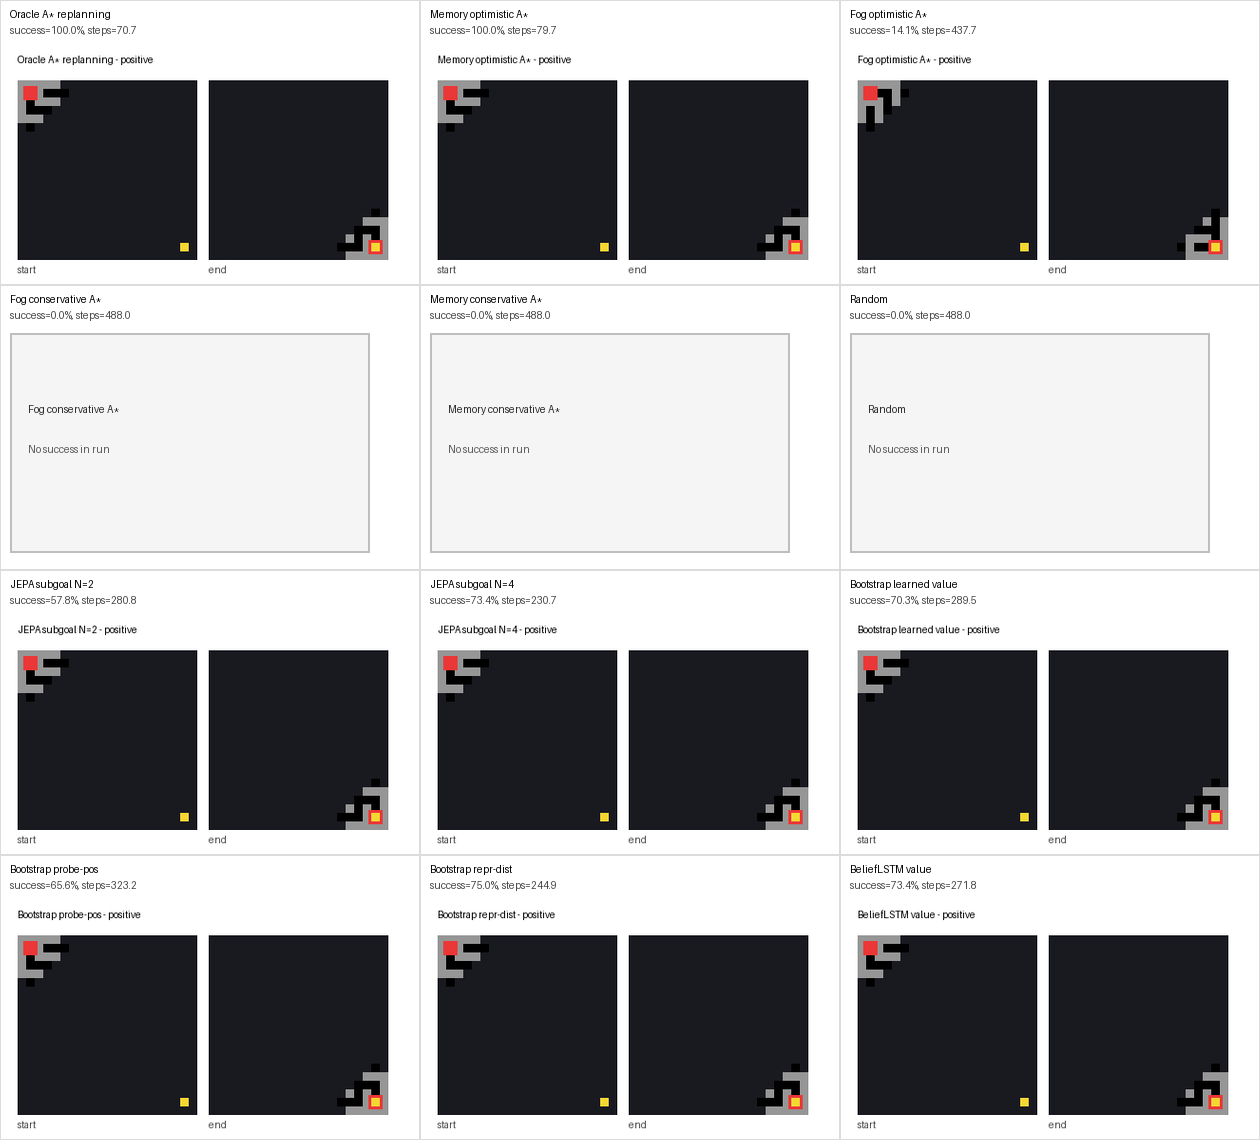
\includegraphics[width=\linewidth]{figures/contact_positive.png}
\end{center}

\section*{Failure Examples}
\begin{center}
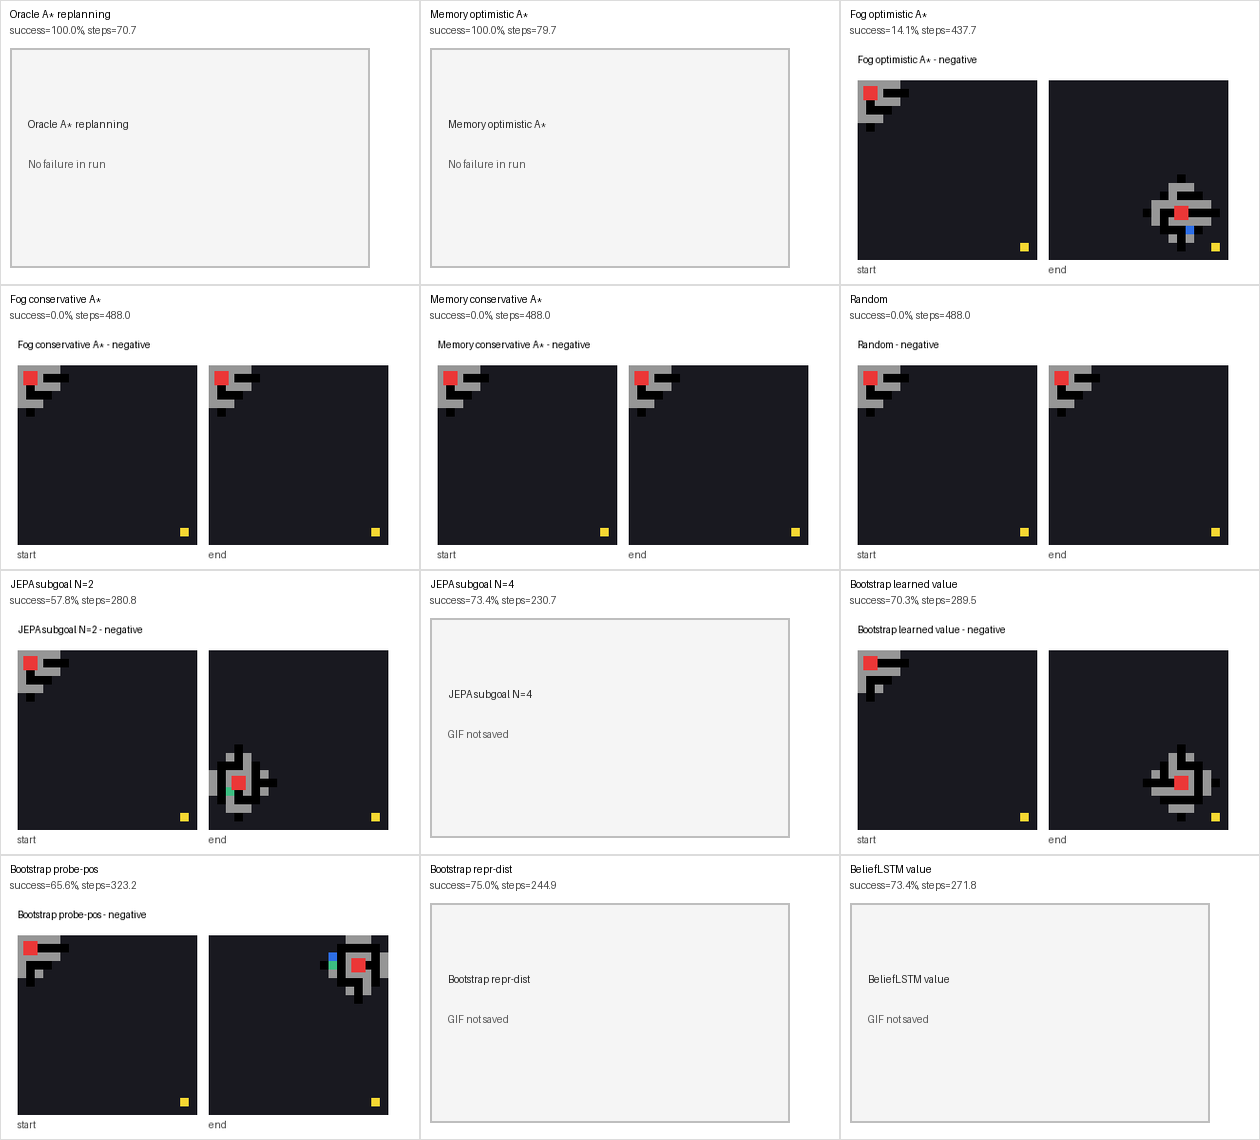
\includegraphics[width=\linewidth]{figures/contact_negative.png}
\end{center}

\section*{GIF Links}
\begin{longtable}{p{0.42\linewidth}ll}
\toprule
Method & Success & Failure \\
\midrule
Oracle A* replanning & \href{run:gifs/oracle_replan/positive.gif}{success GIF} & -- \\
Memory optimistic A* & \href{run:gifs/memory_optimistic/positive.gif}{success GIF} & -- \\
Fog optimistic A* & \href{run:gifs/fog_optimistic/positive.gif}{success GIF} & \href{run:gifs/fog_optimistic/negative.gif}{failure GIF} \\
Fog conservative A* & -- & \href{run:gifs/fog_conservative/negative.gif}{failure GIF} \\
Memory conservative A* & -- & \href{run:gifs/memory_conservative/negative.gif}{failure GIF} \\
Random & -- & \href{run:gifs/random/negative.gif}{failure GIF} \\
JEPA subgoal N=2 & \href{run:gifs/jepa_subgoal_n2/positive.gif}{success GIF} & \href{run:gifs/jepa_subgoal_n2/negative.gif}{failure GIF} \\
JEPA subgoal N=4 & \href{run:gifs/jepa_subgoal_n4/positive.gif}{success GIF} & -- \\
Bootstrap learned value & \href{run:gifs/learned_value/positive.gif}{success GIF} & \href{run:gifs/learned_value/negative.gif}{failure GIF} \\
Bootstrap probe-pos & \href{run:gifs/probe_pos/positive.gif}{success GIF} & \href{run:gifs/probe_pos/negative.gif}{failure GIF} \\
Bootstrap repr-dist & \href{run:gifs/repr_dist/positive.gif}{success GIF} & -- \\
BeliefLSTM value & \href{run:gifs/belief_value/positive.gif}{success GIF} & -- \\
\bottomrule
\end{longtable}

\section*{Notes}
\begin{itemize}
\item \textbf{Oracle A* replanning}: Full current grid A* replanning. Strong myopic oracle, not stochastic-optimal.
\item \textbf{Memory optimistic A*}: A* on accumulated visible map, unknown cells treated as free.
\item \textbf{Fog optimistic A*}: A* on current local observation, unknown cells treated as free.
\item \textbf{Fog conservative A*}: A* on current local observation, unknown cells treated as walls.
\item \textbf{Memory conservative A*}: A* on accumulated map, never-seen cells treated as walls.
\item \textbf{Random}: Uniform random cardinal action baseline.
\item \textbf{JEPA subgoal N=2}: A*-distilled waypoint head; A* not queried at eval.
\item \textbf{JEPA subgoal N=4}: A*-distilled longer waypoint head; first saved GIFs are all successes.
\item \textbf{Bootstrap learned value}: A*-free local exploration + hindsight TD value.
\item \textbf{Bootstrap probe-pos}: World-model rollout scored by decoded position distance.
\item \textbf{Bootstrap repr-dist}: World-model rollout scored by latent distance to goal.
\item \textbf{BeliefLSTM value}: Frozen JEPA + recurrent belief state + learned value.
\end{itemize}

\section*{Main Reading}
The strongest non-oracle controller in this batch is still representation
distance in JEPA latent space: it reaches 75.0\% success with 244.9 mean steps.
The BeliefLSTM value improves the first learned value head, reaching 73.4\%
success, but it still makes more blocked moves. The next useful Track 7
iteration should make the learned value explicitly penalize blocked transitions
and use memory signals that distinguish seen-passable, seen-blocked, and
unseen cells.

\end{document}
